\begin{figure}[!p]
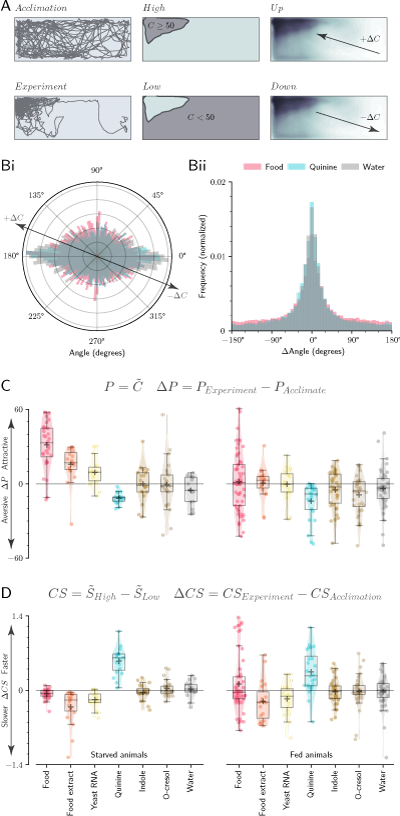
\includegraphics[width=\linewidth]{Figures/images/3.eps}
 \captionof{figure}{\textbf{ Larval exploration behavior is best explained by a chemokinesis search model.} A: Diagram of behavioral quantifications. Larvae were observed during a 15-minute acclimation period in clean water, followed by a 15-minute experiment in the presence of the stimulus. The arena was divided into an area of high (${\geq}$50${\%}$) and low concentration (<50${\%}$). Larvae could move in a direction that increased local concentration (+${\Delta}$C) or decreased local concentration (-${\Delta}$C). Bi: Orientation of animals in the arena throughout the experiment. Larvae did not exhibit directional movement in response to appetitive or aversive stimuli. Note that larvae spend more time moving horizontally (0${\degree}$, 180${\degree}$) because the rectangular arena is longer in the horizontal direction. Bii: Larvae did not change frequency of turns (${\Delta}$angle) in response to appetitive or aversive stimuli. C: Box plots for the population median (${\pm}$ 1 quartile), population mean (+ marker) and mean response for each individual (dots) for larval preference (${\Delta}$P). A horizontal line at 0 represents no change in behavior following stimulus addition. D: As in C, except for stimulus-dependent changes in Concentration-dependent Speed (${\Delta}$CS).
 }
 \label{fig:fig1}
\end{figure}